\documentclass{article}
\usepackage{graphicx} % Required for inserting images
\usepackage{subcaption}
\usepackage{float}
\usepackage{listings}
\usepackage{amsmath}
\usepackage{xcolor}
\title{Computational Linear Algebra Coursework2}
\author{02242457}
\date{December 2024}

\begin{document}
\maketitle

\begin{figure}[ht] % Placement options for the entire figure
    \centering
    \begin{subfigure}[b]{0.45\linewidth} % Width of subfigure
        \centering
        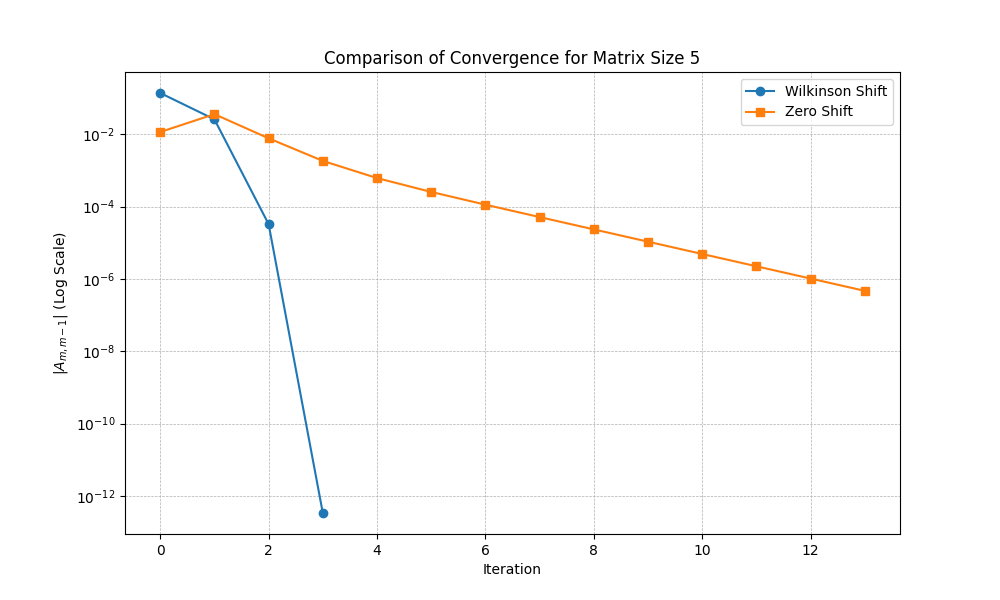
\includegraphics[width=\linewidth]{Comparison_of_Covergence_5.png}
        \caption{Comparison of Convergence when size=5}
        \label{fig:subfig1}
    \end{subfigure}
    \hfill
    \begin{subfigure}[b]{0.45\linewidth} % Width of subfigure
        \centering
        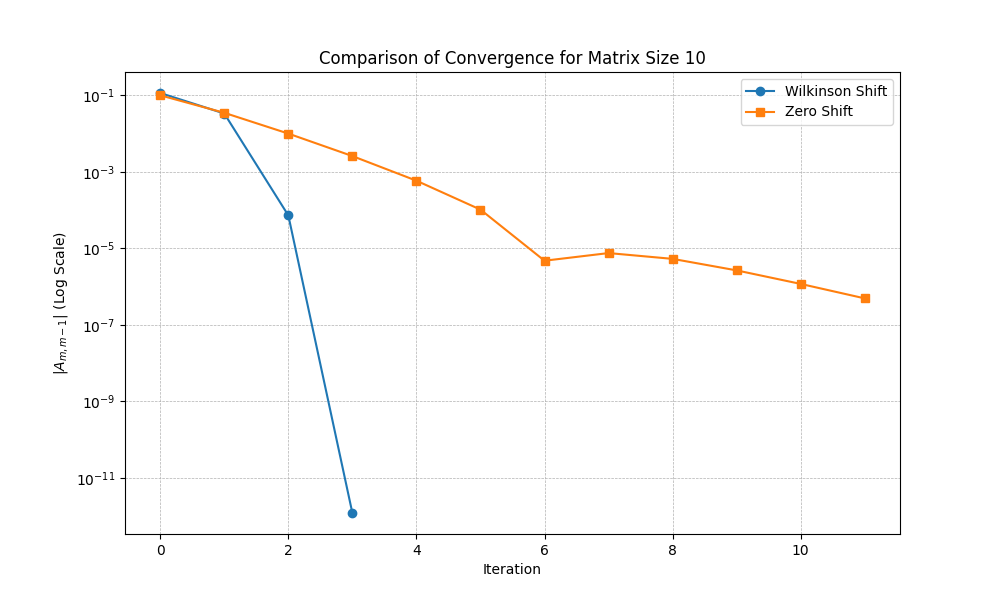
\includegraphics[width=\linewidth]{Comparison_of_convergence_10.png}
        \caption{Comparison of Convergence when size=10}
        \label{fig:subfig2}
    \end{subfigure}
    \caption{Comparison of Convergence}
    \label{fig:combined_fig}
\end{figure}
1.b After adding the optional argument \texttt{use\_zero\_shift}, we can compare the performance by setting \texttt{use\_zero\_shift} to either \texttt{False} or \texttt{True}. When a shift is used, \( |A^{(k)}_{m,m-1}| \) converges to 0 much more quickly. Because the QR algorithm does not focus on any specific eigenvalue, requiring more iterations to minimize the off-diagonal elements. In contrast, the Wilkinson shift achieves significantly faster convergence by offering a more accurate estimation of the eigenvalue near the bottom-right corner. Above are the examples for matrix size=5 and 10.\vspace{0.5cm}
\newline 1.c Define a function called \texttt{find\_eigenvalue} (for now, use the \texttt{triQR} method without shift). For a random matrix of size 10, use \texttt{find\_eigenvalue} to generate a list of its eigenvalues. Then, plug each eigenvalue into the \texttt{inverse\_it} function. Since the input is already close to or is the actual eigenvalue, \texttt{inverse\_it} will return an eigenvalue after 1 or 2 iterations. By comparing these two sets of eigenvalues (expected to show a small difference), we can verify that both methods yield approximately the same eigenvalues. See the example below.\vspace{0.5cm}
\newline Generate a random matrix with size=10 and implement above steps.(see code in cw2\_question1: find\_eigenvalue\_use\_mu and find\_eigenvalue\_with\_mu)

\begin{align*}
&[0.0, 2.220446049250313 \times 10^{-16}, 3.774758283725532 \times 10^{-15}, \\
&1.1102230246251565 \times 10^{-15}, 3.552713678800501 \times 10^{-15}, \\
&1.1102230246251565 \times 10^{-15}, 1.7763568394002505 \times 10^{-15}, \\
&8.881784197001252 \times 10^{-16}, 2.6645352591003757 \times 10^{-15}, \\
&2.6645352591003757 \times 10^{-15}]
\end{align*}
all differences of two eigenvalues are nearly 0, align with the conclusion.\vspace{0.5cm}
\newline 1.d Modified the \texttt{find\_eigenvalue} with\texttt{ use\_zero\_shift=False} and add a new return iterate\_time to both of functions. For a matrix, print their iterations respectively. See examples below and the graph with size changing.(the first iteration times comes from function without shift while the second is with shift.)
\newline For a matrix of size \(10\): \(1910 \quad 20\) \\
For a matrix of size \(100\): \(7237 \quad 184\) \vspace{0.5cm}
\newline The first number is significantly larger than the second, indicating using shift will have a massive improve of efficiency and computing cost.
\begin{figure}[H]
    \centering
    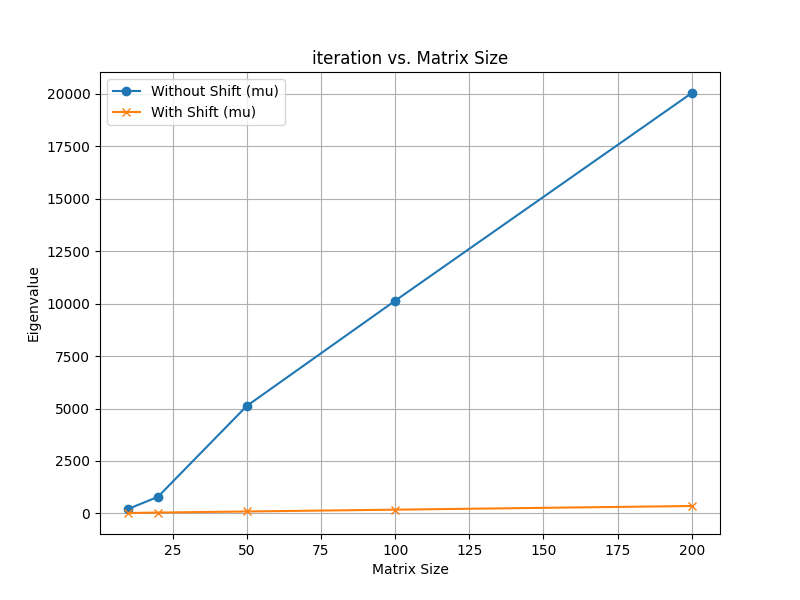
\includegraphics[width=0.75\linewidth]{iteration_times_compare.png}
    \caption{iteration vs matrix size}
    \label{fig:enter-label}
\end{figure}
iteration vs matrix size figure shows that with size increasing, iteration times of use\_shift remains under 500 and rise slowly while the other increases dramatically. The difference between two methods getting bigger. With a large size matrix, the use\_shift function will be more efficient compared to the other.
\begin{figure}[H]
    \centering
    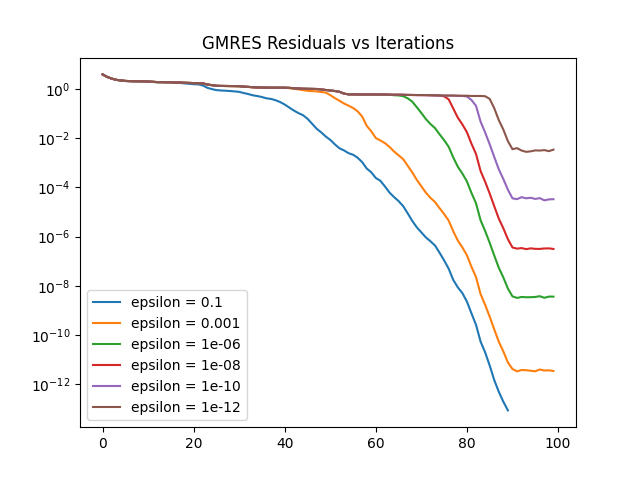
\includegraphics[width=0.75\linewidth]{GMRES_IT.png}
    \caption{GMRES residual norm vs iteration}
    \label{fig:GMRES vs iteration}
\end{figure}

2.a When $\epsilon$ is large (matrix is not ill-conditioned), residual norm decreases means A converges efficiently using GMRES. However when $\epsilon$ goes to 0(1e-12 for example), the matrix converges slower and the residual norm reaches the plateaus around 0.1 at 90 iterations which is prominently larger than our tolerance.
\begin{figure}[ht] % Placement options for the entire figure
    \centering
    \begin{subfigure}[b]{0.45\linewidth} % Width of subfigure
        \centering
        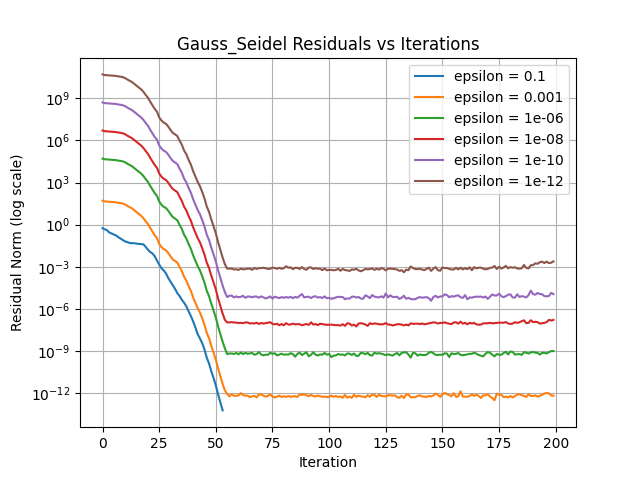
\includegraphics[width=\linewidth]{GS_IT.png}
        \caption{GS residual norm vs iteration}
        \label{fig:subfig1}
    \end{subfigure}
    \hfill
    \begin{subfigure}[b]{0.45\linewidth} % Width of subfigure
        \centering
        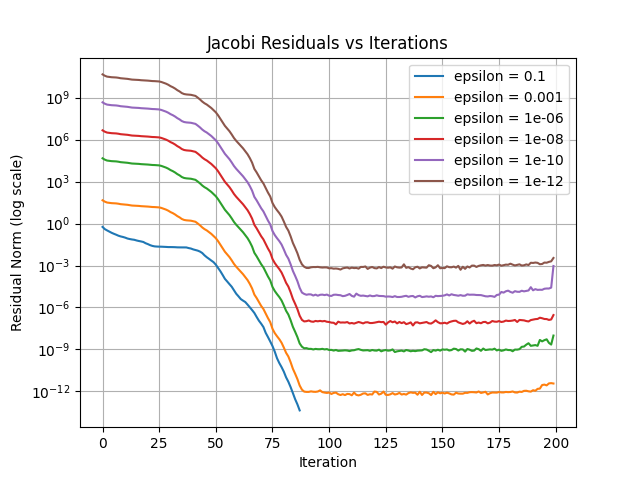
\includegraphics[width=\linewidth]{Jacobi_IT.png}
        \caption{Jacobi residual norm vs iteration}
        \label{fig:subfig2}
    \end{subfigure}
    \caption{Overall caption for the figure}
    \label{fig:combined_fig}
\end{figure}
\newline 2.(b)(c)For matrix with larger size(the examples use size as 100) and ill-conditioned, GS and Jacobi will perform better compared with original GMRES for all epsilons. Generally with precondition the final residual will be smaller than GMRES without precondition and less iterations. GMRES iterates around 90 times to reach plateaus while Jacobi iterates 50 times and GS iterates 85 times.
\end{document}


